\documentclass{standalone}
\usepackage{tikz}
\usepackage{ctex,siunitx}
\setCJKmainfont{Noto Serif CJK SC}
\usepackage{tkz-euclide}
\usepackage{amsmath}
\usetikzlibrary{patterns, calc,3d}
\usetikzlibrary {decorations.pathmorphing,decorations.pathreplacing,decorations.shapes}
\tikzset{label style/.append style={font=\small}}
\begin{document}
\small
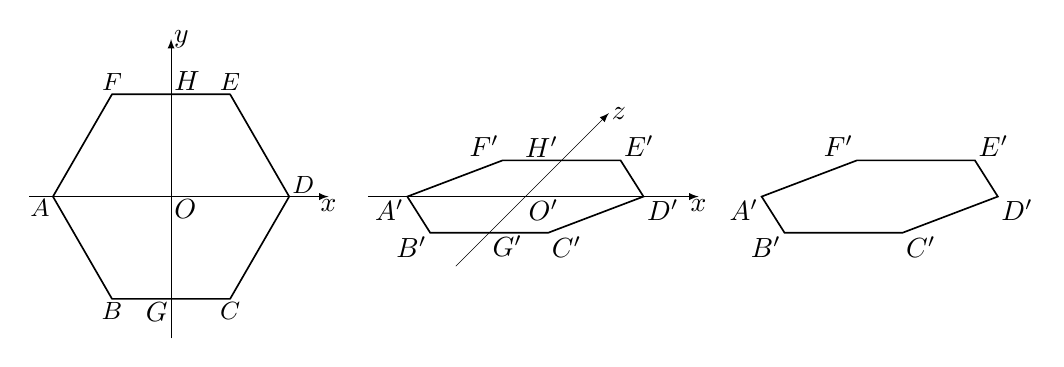
\begin{tikzpicture}[>=latex,scale=1.0,inner sep=1pt]
  \begin{scope}
    \draw[very thin,->](-1.8,0)--(2,0)node[below]{$x$};
    \draw[very thin,->](0,-1.8)--(0,2)node[right]{$y$};
    \node at (0,0)[below right]{$O$};
    \foreach \x[count=\i from 3] in {A,B,C,D,E,F}
    { \tkzDefPoint(\i*60:1.5){\x}}
    \tkzDrawPolygon[semithick](A,B,C,D,E,F)
    \tkzLabelPoints[above](E,F)
    \tkzLabelPoints[above right](D)
    \tkzLabelPoints[below left](A)
    \tkzLabelPoints[below](B,C)
    \node at (0,{0.75*sqrt(3)})[above right]{$H$};
    \node at (0,{-0.75*sqrt(3)})[below left]{$G$};
  \end{scope}
  \begin{scope}[xshift=4.5cm,z={(45:5mm)},canvas is zx plane at y=0]
    \draw[very thin,->](0,-2)--(0,2.2)node[below]{$x$};
    \draw[very thin,->](-2.5,0)--(3,0)node[right]{$z$};
    \draw[semithick]
      (30:1.5)node[above right]{$E'$}--
      (90:1.5)node[below right]{$D'$}--
      (150:1.5)node[below right]{$C'$}--
      (210:1.5)node[below left]{$B'$}--
      (270:1.5)node[below left]{$A'$}--
      (330:1.5)node[above left]{$F'$}--cycle;
    \node at (0,0)[below right]{$O'$};
    \node at ({0.75*sqrt(3)},0)[above left]{$H'$};
    \node at ({-0.75*sqrt(3)},0)[below right]{$G'$};
  \end{scope}
  \begin{scope}[xshift=9cm,z={(45:5mm)},canvas is zx plane at y=0]
    \draw[semithick]
      (30:1.5)node[above right]{$E'$}--
      (90:1.5)node[below right]{$D'$}--
      (150:1.5)node[below right]{$C'$}--
      (210:1.5)node[below left]{$B'$}--
      (270:1.5)node[below left]{$A'$}--
      (330:1.5)node[above left]{$F'$}--cycle;
  \end{scope}
\end{tikzpicture}
\end{document}